\documentclass[fleqn]{beamer}

\usepackage{amsmath}
\usepackage{animate}
\usepackage{amsfonts}
\usepackage[mathscr]{eucal}
\usepackage{subcaption}
\usepackage{wrapfig}
\usepackage{graphicx}

\usepackage{fancyhdr}
\usepackage{pstricks}
\usepackage{pst-func}
\usepackage{pst-plot}
\usepackage[utf8x]{inputenc}
\usepackage[spanish]{babel}


\setbeamertemplate{navigation symbols}{}
\definecolor{UniBlue}{RGB}{83,121,170}
\setbeamercolor{frametitle}{fg=black,bg=white}
\setbeamercolor{title}{fg=black,bg=yellow!85!orange}
%\setbeamercolor{title}{fg=red,bg=yellow!90!blue}
\usetheme{Madrid}

\beamersetuncovermixins{\opaqueness<1>{25}}{\opaqueness<2->{15}}
\begin{document}

\title{CGeIHC}
\author{Reynaldo Martell}
\date{\today} 

\begin{frame}
\titlepage
\end{frame}

\begin{frame}\frametitle{\rule{0mm}{10mm}\rule{5mm}{0mm} Computación Gráfica. }
Laboratorio de Proyectos Externos 2, Planta Baja, Edificio U - "Bernardo
Quintana Arrioja“, Facultad de Ingeniería
\begin{figure}[H]
	\centering
	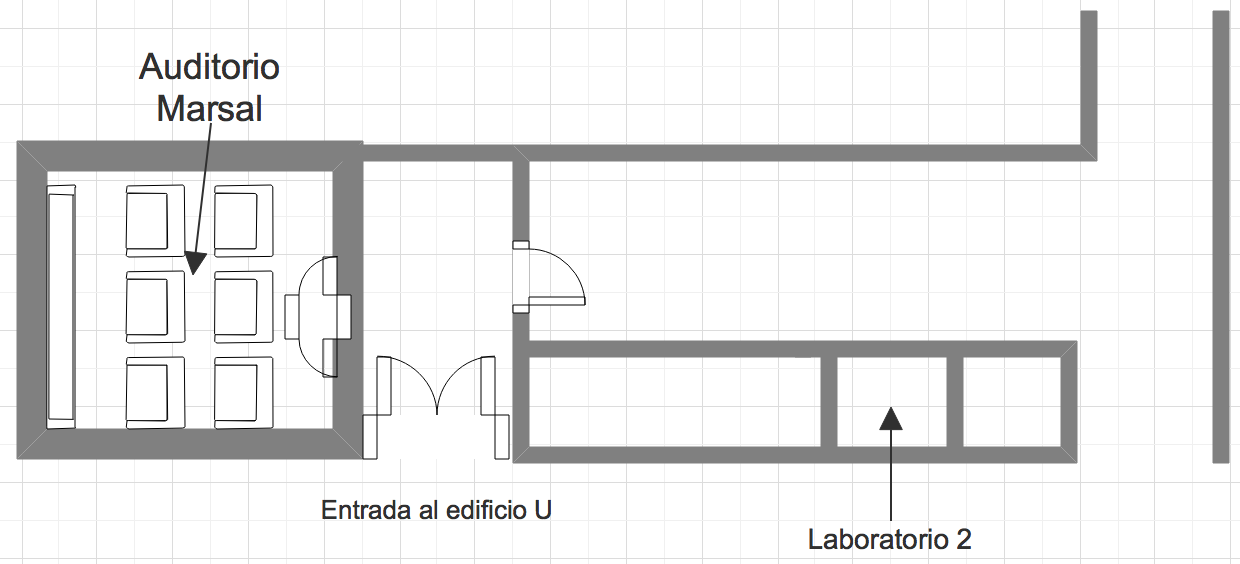
\includegraphics[width=1.0\textwidth]{images/mapa.png}
	\label{mapa}
\end{figure}
\end{frame}

\begin{frame}\frametitle{\rule{0mm}{10mm}\rule{5mm}{0mm} Computación Gráfica. }
\begin{enumerate}
	\item Conceptos matemáticos.
	\item Algoritmos de graficación.
	\item OpenGL 4.0
	\item Visual studio 2017 (Windows) o Eclipse kepler (Ubuntu)
\end{enumerate}
\end{frame}

\begin{frame}\frametitle{\rule{0mm}{10mm}\rule{5mm}{0mm} Evaluación. }
\begin{enumerate}
	\item Exámenes 35 \%
	\begin{enumerate}
		\item Parcial 1
		\item Parcial 2
	\end{enumerate}
	\item Proyecto	35 \%
	\item Laboratorio 20\%
	\item Tareas e Investigaciones 10 \%	
\end{enumerate}
\end{frame}

\begin{frame}\frametitle{\rule{0mm}{10mm}\rule{5mm}{0mm} Evaluación - Consideraciones. }
\begin{enumerate}
	\item No tienen derecho a NP aquellos alumnos que presenten alguno de los
exámenes parciales o el final.
	\item Requisito aprobar el laboratorio.
	\item Se exenta del examen final si el promedio es mayor a 6
	\item El final se presenta únicamente si se aprobó el laboratorio y se entrego el
proyecto. Se tomará la siguiente evaluación.
	\begin{enumerate}
		\item Examen final 60\%
		\item Proyecto 30 \%
		\item Laboratório 10 \%
	\end{enumerate}
\end{enumerate}
\end{frame}

\begin{frame}\frametitle{\rule{0mm}{10mm}\rule{5mm}{0mm} Evaluación - Fechas importantes. }
\begin{enumerate}
	\item Primer parcial. 18 de Septiembre.
	\item Segundo parcial. 13 de Noviembre.
	\item Entrega de proyecto. 27 de Noviembre.
	\item Examen final. 2 de Diciembre.
\end{enumerate}
\end{frame}

\begin{frame}\frametitle{\rule{0mm}{10mm}\rule{5mm}{0mm} Tarea. }
\begin{enumerate}
	\item Tarea inscribirse al grupo: \hfill \break
	https://groups.google.com/d/forum/cgeihc-2020-1
	\item Github.
	\begin{enumerate}
		\item Definición.
		\item ¿Qué es un branch?
		\item ¿Qué es un fork?
		\item Utilidad.
		\item Comandos básicos.
		\item Crear cuenta y crear su primer repositorio.
	\end{enumerate}
	\item Instalar las herramientas para el desarrollo.
	\begin{enumerate}
		\item Visual Studio 2017 Windows
		\item Software/Git-2.9.2-64-bit.rar
		\item Software/TortoiseGit-2.2.0.0-64bit.rar
	\end{enumerate}
\end{enumerate}
\end{frame}

\end{document}

